\documentclass[10pt]{amsart}
\usepackage[margin=1.4in]{geometry}
\usepackage[usenames,dvipsnames,cmyk]{xcolor} %load first
\usepackage{cancel}
\usepackage{graphicx,subfig}
\graphicspath{ {./images/} }

\usepackage{amssymb,amsmath,enumitem,url}

\newcommand{\D}{\mathrm{d}}
\newcommand{\I}{\mathrm{i}}
\DeclareMathOperator{\E}{e}
\DeclareMathOperator{\OO}{O}
\DeclareMathOperator{\oo}{o}
\DeclareMathOperator{\erfc}{erfc}
\DeclareMathOperator{\real}{Re}
\DeclareMathOperator{\imag}{Im}
\usepackage{tikz}
\usepackage[framemethod=tikz]{mdframed}
\theoremstyle{nonumberplain}

\mdtheorem[innertopmargin=-5pt]{sol}{Solution}
%\newmdtheoremenv[innertopmargin=-5pt]{sol}{Solution}
\definecolor{MichiganBlue}{HTML}{00274C}
\definecolor{MichiganYellow}{HTML}{FFCB05}  
\definecolor{NicePurple}{RGB}{75,56,76} %PrincePurple
\definecolor{NiceRed}{RGB}{230,37,52}
\definecolor{MidnightBlue}{rgb}{0.1, 0.1, 0.44}
\usepackage[colorlinks=true, linkcolor=MidnightBlue, citecolor=MidnightBlue, urlcolor=MidnightBlue]{hyperref}

\begin{document}
\pagestyle{empty}

\newcommand{\mline}{\vspace{.2in}\hrule\vspace{.2in}}

\noindent
\text{Hunter Lybbert} \\
\text{Student ID: 2426454} \\
\text{10-21-24} \\
\text{AMATH 567} \\

\title{\bf { Homework 4} }


\maketitle
\noindent
Collaborators*: Nate Ward, Erin, Hailey, Laura..., Cooper, Jenny \\
\\
\tiny
\text{*Listed in no particular order. And anyone I discussed at least part of one problem with is considered a collaborator.}
\normalsize
\mline
\noindent
\textbf{TODO:} Now that you know the `$\I$' symbol exists, consider changing each of the `$i$' characters to `$\I$' characters.
\begin{enumerate}[label={\bf {\arabic*}:}]
\item From A\&F: 2.4.2 c, e.\\
Evaluate the integral $\oint_Cf(z)\D z$, where C is the unit circle enclosing the origin, and $f(z)$ is given as follows: \\
c) $$f(z) = \frac {1} {\bar z}$$
\textit{Solution:} \\
We want to evaluate
$$
\oint_C\frac {1} {\bar z} \D z
$$
on the parameterized unit circle $z = \E^{i\theta}$ where $\theta \in [0, 2\pi)$, where $\bar z = \E^{-i\theta}$ on the unit circle.
Note, before we do the substitution we need $\D z = i\E^{i\theta} \D \theta$. Now our integral is
\begin{align*}
\oint_C\frac {1} {\bar z} \D z &= \int_0^{2\pi}\frac {1} {\E^{-i\theta}} i\E^{i \theta}\D \theta \\
					  &= \int_0^{2\pi} i \E^{2i \theta} \D \theta \\
					  &= \left( \left. \frac 1 2 \E^{2i\theta} \right|_0^{2\pi}\right) \\
					  &= \frac 1 2 \E^{4\pi i} - \frac 1 2 \E^{0} \\
					  &= \frac 1 2 - \frac 1 2 \\
					  &= 0
\end{align*}
\qed
\\
e) $$f(z) = \E^{\bar z}$$
\textit{Solution:} \\
We will use the same substitutions from the previous part
\begin{align*}
\oint_C\E^{\bar z} \D z &= \int_0^{2\pi}\E^{\E^{-i\theta}} i\E^{i \theta}\D \theta \\
				  &= \int_0^{2\pi} \sum_{j=0}^{\infty} \frac{\left(\E^{-i\theta}\right)^j}{j!} i\E^{i\theta} \D \theta \\
				  &= \sum_{j=0}^{\infty} \int_0^{2\pi} i \frac{\left(\E^{-i\theta}\right)^j}{j!} {\E^{i\theta}} \D \theta.
\end{align*}
We are justified in reordering the integral of the infinite sum to be the infinite sum of the integrals since the original series converges absolutely.
Notice we can pull out the first term where $j=1$ to get,
$$
\sum_{j=0}^{\infty} \int_0^{2\pi} i \frac{\left(\E^{-i\theta}\right)^j}{j!} {\E^{i\theta}} \D \theta
= \int_0^{2\pi} i \frac{\left(\E^{-i\theta}\right)^0}{0!} {\E^{i\theta}} \D \theta
+ \int_0^{2\pi} i \frac{\left(\E^{-i\theta}\right)^1}{1!} {\E^{i\theta}} \D \theta
+ \sum_{j=2}^{\infty} \int_0^{2\pi} i \frac{\left(\E^{-i\theta}\right)^j}{j!} {\E^{i\theta}} \D \theta.
$$
We need to look more closely at this first two terms, observe
\begin{align*}
\int_0^{2\pi} i \frac{\left(\E^{-i\theta}\right)^0}{0!} {\E^{i\theta}} \D \theta
= \int_0^{2\pi} i \E^{i\theta} \D \theta
= \left. \E^{i\theta} \right|_0^{2\pi}
= \E^{i2\pi} - \E^{0}
= 0
\end{align*}
and
\begin{align*}
\int_0^{2\pi} i \frac{\left(\E^{-i\theta}\right)^1}{1!} \E^{i\theta} \D \theta = \int_0^{2\pi} i \frac{\E^{-i\theta}\E^{i\theta}}{1!} \D \theta = \int_0^{2\pi} i \frac{1}{1} \D \theta = i\int_0^{2\pi}\D \theta = 2\pi i.
\end{align*}
Now, I will focus on the integral inside the sum where $j = 2, 3, 4, ...$
\begin{align*}
\int_0^{2\pi} i \frac{\left(\E^{-i\theta}\right)^j}{j!} {\E^{i\theta}} \D \theta &= \int_0^{2\pi} i \frac{\E^{-i\theta j}\E^{i\theta}}{j!} \D \theta \\
	&= \int_0^{2\pi} i \frac{\E^{-i\theta j + i\theta}}{j!} \D \theta \\
	&= \int_0^{2\pi} i \frac{\E^{i\theta\left( - j + 1\right)}}{j!} \D \theta \\
	&= \int_0^{2\pi} \frac{i\E^{i\theta\left(1 - j\right)}}{j!} \D \theta \\
	&= \left. \frac{1}{1 - j} \frac{i\E^{i\theta\left(1 - j\right)}}{j!} \right|_0^{2 \pi} \\
	&= \frac{1}{1 - j} \frac{i\E^{i2\pi\left(1 - j\right)}}{j!} - \frac{1}{1 - j} \frac{i\E^0}{j!} \\
	&= \frac{i}{\left(1 - j\right)j!}\left(\E^{i2\pi\left(1 - j\right)} - 1 \right) \\
	&= \frac{i}{\left(1 - j\right)j!}\left(1 - 1 \right) \\
	&= 0. \\
\end{align*}
I want to clarify why $\E^{i2\pi\left(1 - j\right)} = 1$.
Since $j \in \{2, 3, ...\}$, then $1 - j$ is an integer and we have $\E^{i2\pi \ell}$ where $\ell \in \mathbb Z$, thus $\E^{i2\pi \ell} = 1$.
Now we return to the original problem
$$
\sum_{j=0}^{\infty} \oint_0^{2\pi} i \frac{\left(\E^{-i\theta}\right)^j}{j!} {\E^{i\theta}} \D \theta = 0 + 2\pi i + \sum_{j=2}^{\infty} 0 = 2\pi i.
$$
Now we have completed the requisite task.
\qed
\\

\item From A\&F: 2.4.4 a, b.
Use the principal branch where the argument is in $[-\pi,\pi)$.
Discuss any ambiguities. 
Use the principal branch of $\log(z)$ and $z^{\frac{1}{2}}$ where the argument is in $[-\pi,\pi)$ to evaluate the following: \\
a) $$\int_{-1}^{1}\log z \D z$$
\textit{Solution:} \\
We want to parameterize this once again using $z = r\E^{i\theta}$ where $\theta \in [-\pi,\pi)$. Now our integral is
\begin{align*}
\int_{-1}^{1}\log z \D z &= \int_{-\pi}^{0}\log \left(\E^{i\theta}\right) i \E^{i\theta} \D \theta \\
	&= \int_{-\pi}^{0} i\theta i \E^{i\theta} \D \theta.
\end{align*}
Let's use integration by parts, woohoo! We will assign the substitutions as follows:
\begin{align*}
u &= i\theta \\
\D u &= i \D \theta\\
\\
\D v &= i\E^{i \theta} \D \theta \\
v &= \E^{i \theta}.
\end{align*}
Plugging this in we have
\begin{align*}
\int_{-\pi}^{0} i\theta i \E^{i\theta} \D \theta &= \left. i\theta \E^{i\theta}\right|_{-\pi}^0 - \int_{-\pi}^0 i \E^{i \theta} \D \theta \\
	&= \left(0 - \left(-i\pi \E^{-i\pi}\right)\right) - \left. \E^{i\theta}\right|_{-\pi}^0 \\
	&= 0 + i\pi \E^{-i\pi} - \left. \E^{i\theta}\right|_{-\pi}^0 \\
	&= i\pi \E^{-i\pi} - \left(\E^{0} - \E^{-i\pi} \right) \\
	&= - i\pi - \left(1 - \left( - 1 \right) \right) \\
	&= - i\pi - \left(2\right) \\
	&= - i\pi - 2. \\
\end{align*}
\qed
\\
b) $$\int_{-1}^{1}z^{\frac{1}{2}} \D z$$
\textit{Solution:} \\
We want to parameterize this once again using $z = r\E^{i\theta}$ where $\theta \in [-\pi,\pi)$. Now our integral is
\begin{align*}
\int_{-1}^{1} z^{\frac{1}{2}} \D z &= \int_{-\pi}^{0} \left(\E^{i\theta}\right)^{\frac{1}{2}} i \E^{i\theta} \D \theta \\
	&= \int_{-\pi}^{0} i\E^{\frac{i\theta}{2}} \E^{i\theta} \D \theta \\
	&= \int_{-\pi}^{0} i\E^{\frac{i3}{2}\theta} \D \theta \\
	&= \left. \frac 2 3 \E^{\frac{i3}{2}\theta} \right|_{-\pi}^{0} \\
	&= \frac 2 3 \E^{ - \frac{i3}{2} \pi} - \frac 2 3. \\
\end{align*}
Now remembering our branch cut limits $\theta$ to be within $[-\pi, \pi)$ we change the angle $-\frac 3 2 \pi$ to be $\frac 1 2 \pi$.
Hence,
\begin{align*}
\frac 2 3 \E^{ - \frac{i3}{2} \pi} - \frac 2 3 &= \frac 2 3 \E^{ - \frac{i2}{2} \pi} \E^{ - \frac{i\pi}{2}} - \frac 2 3 \\
	&= \frac 2 3 \E^{ \frac{i\pi}{2}} - \frac 2 3 \\
	&= \frac 2 3 \left( i - 1\right).
\end{align*}
\qed
\\
\item From A\&F: 2.4.7 \\
Let C be an open (upper) semicircle of radius $R$ with its center at the origin, and consider $\int_C f(z) \D z$.
 Let $f(z) = \frac{1}{z^2 + a^2}$ for a real $a > 0$.
Show that $\left| f(z) \right| \leq \frac{1}{R^2 - a^2}$, $R > a$, and
$$
\left| \int_C f(z) dz \right| \leq \frac{\pi R}{R^2 - a^2}, \quad R > a.
$$
\textit{Solution:} \\
First, we want to show
$$
\left| f(z) \right| \leq \frac{1}{R^2 - a^2}
$$
where $R > a > 0$ and a $\in \mathbb R$.
Let's consider the function more closely
\begin{align*}
f(z) =  \frac{1}{z^2 + a^2} &= \frac{1}{(x + \I y)^2 + a^2} \\
	&= \frac{1}{x^2 + 2ixy - y^2 + a^2} \\
	&= \frac{1}{x^2 - y^2 + a^2 + i2xy }. \\
\end{align*}
Notice, we can write the real and imaginary parts of the complex number in the denominator as functions $u(x, y)$ and $v(x, y)$.
Where $u(x, y) = x^2 - y^2 + a^2$ and $v(x, y) = 2xy$.
Now we get 
$$
f(z) = \frac{1}{x^2 - y^2 + a^2 + i2xy }	 = \frac{u - iv }{u - iv }\frac{1}{u + iv } = \frac{u - iv }{u^2 + v^2 }.
$$
Then we calculate
\begin{align*}
\left| f(z) \right| &= \left| \frac{u - iv }{u^2 + v^2 } \right| \\
	&= \left| \frac{u }{u^2 + v^2 } - i\frac{v}{u^2 + v^2 } \right| \\
	&= \sqrt{
		\left(\frac{u }{u^2 + v^2 }\right)^2 + \left(\frac{v }{u^2 + v^2 }\right)^2
	} \\
	&= \sqrt{
		\frac{u^2 }{\left( u^2 + v^2 \right)^2} + \frac{v^2 }{\left( u^2 + v^2 \right)^2}
	} \\
	&= \sqrt{
		\frac{u^2 + v^2 }{\left( u^2 + v^2 \right)^2}
	} \\
	&= \sqrt{
		\frac{1}{u^2 + v^2}
	} \\
	&= \frac{1}{\sqrt{u^2 + v^2}}.
\end{align*}
If we plug our substitution back in we see
\begin{align*}
\frac{1}{\sqrt{u^2 + v^2}} &= \frac{1}{\sqrt{\left(x^2 - y^2 + a^2 \right)^2 + \left(2xy \right)^2}} \\
	&= \frac{1}{\sqrt{\left(x^2 - y^2 + a^2 \right)\left(x^2 - y^2 + a^2 \right) + 4x^2y^2}} \\
	&= \frac{1}{
		\sqrt{
			x^4 - x^2y^2 + x^2a^2 -x^2y^2 + y^4 - y^2a^2 + x^2a^2 - y^2a^2 + a^4 + 4x^2y^2
		}
	} \\
	&= \frac{1}{
		\sqrt{
			x^4 + x^2a^2 + y^4 - y^2a^2 + x^2a^2 - y^2a^2 + a^4 + 2x^2y^2
		}
	}.
\end{align*}
Now we add zero in a particular fashion, namely $- 4x^2a^2 + 4x^2a^2 $, so we can regroup the terms and refactor to get closer to what we desire
\begin{align*}
	&= \frac{1}{
		\sqrt{
			x^4 + y^4 - y^2a^2 + 2x^2a^2 - y^2a^2 + a^4 + 2x^2y^2 +\left( - 4x^2a^2 + 4x^2a^2 \right)
		}
	} \\
	&= \frac{1}{
		\sqrt{
			x^4 + y^4 - 2y^2a^2 + a^4 + 2x^2y^2 - 2x^2a^2 + 4x^2a^2
		}
	} \\
	&= \frac{1}{\sqrt{\left(x^2 + y^2 - a^2\right)^2 + \left(2xa\right)^2}}.
\end{align*}
Using the fact that $\sqrt{a + b} \geq \sqrt{a}$ for $a, b > 0$, in our next step we get a smaller denominator which makes the overall expression greater or equal to the previous step. Note, equality only holds when $x=0$.
\begin{align*}
 \frac{1}{\sqrt{\left(x^2 + y^2 - a^2\right)^2 + \left(2xa\right)^2}}
 	&\leq \frac{1}{\sqrt{\left(x^2 + y^2 - a^2\right)^2}} \\
	&= \frac{1}{x^2 + y^2 - a^2} \\
	&= \frac{1}{|z|^2 - a^2} \\
	&= \frac{1}{R^2 - a^2}
\end{align*}
Therefore $\left| f(z) \right| \leq \frac{1}{R^2 - a^2}$. \\
\qed

\noindent
Next we wish to show that 
$$
\left| \int_C f(z) dz \right| \leq \frac{\pi R}{R^2 - a^2}, \quad R > a.
$$
By Theorem 2.4.2 from A\&F, if $f(z)$ is continuous on contour C, then
$$
\left| \int_C f(z) dz \right| \leq ML
$$
where $L$ is the length of $C$ and $M$ is an upper bound for $\left| f(z) \right|$.
We have that $C$ is continuous, since $a >0$ and $a < R$ and there are no singularities or weirdness with $f(z)$ on the specified contour.
So we have 
$$
M = \frac{1}{R^2 - a^2}
$$
as we calculated in the first part of this problem.
Additionally, we know the arc length of $C$ is easy to calculate because it is half the circumference of the circle with radius $R$.
To convince myself of this I will show the general arc length formula also provides this quick calculation.
Let our parameterization of this contour be $$z(\theta) = R\E^{i\theta}$$ where $\theta \in [0, \pi)$. Then $$z^\prime(\theta) = Ri\E^{i\theta} = -R\sin\theta + iR\cos\theta.$$
Therefore calculating arc length is as follows,
\begin{align*}
L &= \int_a^b |z^\prime(t)| \D t \\
	&= \int_{0}^{\pi} \left| -R\sin\theta + iR\cos\theta \right| \D \theta \\
	&= \int_{0}^{\pi} \sqrt{ R^2\sin^2\theta + R^2\cos^2\theta } \D \theta \\
	&= \int_{0}^{\pi} \sqrt{ R^2\left(\sin^2\theta + \cos^2\theta\right) } \D \theta \\
	&= \int_{0}^{\pi} R \D \theta \\
	&= \pi R.
\end{align*}
Which is the same as half the circumference ($\frac 1 2 2\pi R = \pi R$).
And thus
$$
\left| \int_C f(z) dz \right| \leq ML \leq \frac{1}{R^2 - a^2} \pi R = \frac{\pi R}{R^2 - a^2}.
$$
Hence, 
$$
\left| \int_C f(z) dz \right| \leq \frac{\pi R}{R^2 - a^2}
$$
as desired.
\qed
\\
\item From A\&F: 2.4.8 \\
Let $C$ be an arc of the circle $\left|z\right| = R$ with $(R > 1)$ of angle $\frac{\pi}{3}$.
Show that 
$$
\left| \int_C \frac{\D z}{z^3 + 1} \right| \leq \frac \pi 3 \left( \frac{R}{R^3 - 1} \right)
$$
and deduce
$$
\lim_{R \rightarrow \infty} \int_C \frac{\D z}{z^3 + 1} = 0
$$
\textit{Solution:} \\
Similar to the previous problem, we will utilize Theorem 2.4.2 from A\&F.
We are justified in this, since the contour $C$ is continuous on the arc of the circle $|z| = R$.
This time, our arc length of the contour $C$ is
$$
L = \frac 1 6 2\pi R = \frac{\pi}{3} R.
$$
Next, we need to calculate $M$ as the upper bound for $\left| \frac{1}{z^3 + 1} \right|$.
Let's use a simpler method than in problem 3. Let's get on with it
$$
\left| f(z) \right| = \left| \frac 1 {z^3 + 1} \right| = \frac 1 {\left|z^3 + 1\right|}.
$$
Notice, if we can get a lower bound for the denominator then we will have an upper bound for the whole expression. It falls out quickly using the parameterization $z = R\E^{i\theta}$ and applying the inverse triangle inequality.
\begin{align*}
\left| z^3 + 1\right| &= \left| R^3\E^{i3\theta} + 1\right| \\
	&= \left| R^3\E^{i3\theta} - \left(-1\right)\right| \\
	&\geq \left| \left|R^3\E^{i3\theta}\right| - \left|\left(-1\right)\right|\right| \\
	&= \left| R^3 - 1\right| \\
	&= R^3 - 1
\end{align*}
where the last equality holds because $R > 1$.
Therefore, we have our lower bound for the denominator
$$
\left| z^3 + 1\right| \geq R^3 - 1,
$$
and thus an upper bound for the expression
$$
\left|f(z)\right| = \frac 1 {\left| z^3 + 1\right|} \leq \frac 1 {R^3 - 1} = M.
$$
Finally, applying Theorem 2.4.2 from A\&F we have
$$
\left| \int_C f(z) dz \right| \leq ML \leq \frac {\pi}{3} R\frac{1}{R^3 - 1} = \frac {\pi}{3} \left(\frac{R}{R^3 - 1}\right).
$$
Hence,
$$
\left| \int_C f(z) dz \right| \leq \frac {\pi}{3} \left(\frac{R}{R^3 - 1}\right).
$$
\qed \\
We will now take the limit of both sides of this inequality as $R$ goes to $\infty$
$$
\lim_{R \rightarrow \infty} \left| \int_C f(z) dz \right|
\leq \lim_{R \rightarrow \infty} \frac {\pi}{3} \left(\frac{R}{R^3 - 1}\right) = \frac \infty \infty.
$$
Applying L'Hôpital's rule once, we have
$$
\lim_{R \rightarrow \infty} \frac {\pi}{3} \left(\frac{1}{3R^2 - 1}\right) = 0.
$$
Therefore,
$$
\lim_{R \rightarrow \infty} \left| \int_C f(z) dz \right| \leq 0.
$$
If the limit of the absolute value of something is less than or equal to 0, then the limit of that thing must be zero.
This is the case because the absolute value is a non-negative function, so the ``$\leq 0 $" must be just an equality. Therefore,
$$
\lim_{R \rightarrow \infty} \left| \int_C f(z) dz \right| = 0.
$$
Note this also implies $\lim_{R \rightarrow \infty} -\left| \int_C f(z) dz \right| = 0$.
Now we have that
$$-\left| \int_C f(z) dz \right| \leq \int_C f(z) dz \leq \left| \int_C f(z) dz \right| $$
and thus by the squeeze theorem,
$$\lim_{R \rightarrow \infty} \int_C f(z) dz = 0.$$
\qed
\\

\item From A\&F: 2.5.1 b, e \\
Evaluate $\oint_C f(z)\D z$, where $C$ is the unit circle centered at the origin, and $f(z)$ is given by the following: \\
b) $$f(z) = \E^{z^2}$$ \\
\textit{Solution:} \\
Let's first break $f(z)$ up into real and imaginary parts so we can define $u(x, y)$ and $v(x, y)$ and check if the Cauchy-Riemann (C-R) equations hold.
\begin{align*}
f(z) &= \E^{z^2} \\
	&= \E^{ x^2 + 2ixy - y^2} \\
	&= \E^{x^2}\E^{2ixy}\E^{- y^2} \\
	&= \E^{x^2}\E^{- y^2}\E^{2ixy} \\
	&= \E^{x^2}\E^{- y^2}\left( \cos (2xy) + i \sin (2xy)\right) \\
	&= \E^{x^2}\E^{- y^2}\cos (2xy) + i \E^{x^2}\E^{- y^2}\sin (2xy).
\end{align*}
Then we can assign $u(x, y) = \E^{x^2}\E^{- y^2}\cos (2xy)$ and $v(x, y) = \E^{x^2}\E^{- y^2}\sin (2xy)$.
Now let's calculate the necessary derivatives to verify if $f(z)$ is analytic.
We have
\begin{align*}
\frac {\partial u}{\partial x} &= \E^{-y^2}\left( 2x\E^{x^2}\cos (2xy) - \E^{x^2} \sin (2xy)2y\right) \\
	&= \E^{x^2}\E^{-y^2}\left( 2x\cos (2xy) - \sin (2xy)2y\right)
\end{align*}
and
\begin{align*}
\frac {\partial v}{\partial y} &= \E^{x^2}\left( (-2y)\E^{-y^2}\sin(2xy) + \E^{-y^2}\cos (2xy)2x\right) \\
	&= \E^{x^2}\E^{-y^2}\left( -2y\sin(2xy) + \cos (2xy)2x\right)
\end{align*}
which are equivalent.
Additionally, we get
\begin{align*}
\frac {\partial v}{\partial x} &= \E^{- y^2} \left( 2x\E^{x^2}\sin (2xy) + \E^{x^2}\cos (2xy)2y \right) \\
	&= \E^{x^2}\E^{- y^2} \left( 2x\sin (2xy) + \cos (2xy)2y \right)
\end{align*}
and
\begin{align*}
- \frac {\partial u}{\partial y} &= -\left( \E^{x^2} \left( -2y\E^{- y^2}\cos (2xy) - \E^{- y^2}\sin (2xy)2x \right) \right) \\
	&= - \E^{x^2} \E^{- y^2} \left( -2y\cos (2xy) - \sin (2xy)2x \right) \\
	&= \E^{x^2} \E^{-y^2} \left(2y\cos (2xy) + \sin (2xy)2x \right)
\end{align*}
which are also equal as desired.
Therefore the C-R equations hold and f(z) is analytic everywhere.
Now by the Theorem 2.5.2 from A\&F or Cauchy' Theorem, we can conclude
$$
\oint_C f(z)\D z = \oint_C \E^{z^2} \D z = 0.
$$
\qed 
\\
e) $$f(z) = \frac{1}{2z^2 + 1} $$ \\
\textit{Solution:} \\
We want to calculate the following integral
$$
\oint_C f(z)\D z = \oint_C \frac{1}{2z^2 + 1} \D z.
$$
First, let's break it down using partial fractions
$$
f(z) = \frac{1}{2z^2 + 1} = \frac{-\frac1 2 i}{\sqrt{2}z - i} + \frac{\frac1 2 i}{\sqrt{2}z + i}.
$$
Now to actually calculate the integral we look at
\begin{align*}
\oint_C \frac{1}{2z^2 + 1} \D z &= \oint_C \left(\frac{-\frac1 2 i}{\sqrt{2}z - i} + \frac{\frac1 2 i}{\sqrt{2}z + i} \right)\D z \\
	&= \oint_C \frac{-\frac1 2 i}{\sqrt{2}z - i}\D z + \oint_C\frac{\frac1 2 i}{\sqrt{2}z + i} \D z.
\end{align*}
Each of these integrals is analytic in the region we care about except for at $\frac i {\sqrt{2}}$ and $-\frac i {\sqrt{2}}$ where the denominators are $0$, respectively.
However, we need to eliminate these two singularities by deforming our contour around each of them.
It is important to establish the orientation of these contours now. I am choosing that my starting contour $C$ is clockwise, hence, the ensuing contours $C_1$ and $C_2$ will be counterclockwise.
We take our contour $C$ and deform it such that we reroute it through a channel $t_1$ to circle $C_1$ of radius $\epsilon_1$ around $\frac i {\sqrt{2}} $ and back up through channel $t_2$ returning to the original contour $C$.
Similarly, we deform $C$ to go around $- \frac i {\sqrt{2}}$, by passing through the channel $t_3$ around $- \frac i {\sqrt{2}}$ via $C_2$ (a circle centered at $- \frac i {\sqrt{2}}$ with radius $\epsilon_2$) and back to $C$ through $t_4$. See Figure \ref{fig:f1} for a rough cartoon of how we deform our contour.
\\
\begin{figure}[h]
	\centering
	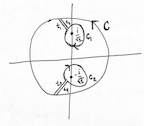
\includegraphics{problem5contour}
	\caption{
		I am including this visual because it helps me make sense of how to eliminate the singularities and use Cauchy's Theorem (Theorem 2.5.2 A\&F) to calculate the integral. I am acknowledging that this graphic is of a poor resolution, I am still figuring out the best ways to include images in \LaTeX. Additionally I should have labeled that the vertical axis is the imaginary ($\Im$) axis and the horizontal axis is the real ($\Re$) axis.
	}\label{fig:f1}
\end{figure}

\noindent
Once we have constructed this deformed contour such that our function $f(z)$ is analytic in a simply connected domain $D$, and along our new contour in $D$, by Cauchy's Theorem we say (I acknowledge an abuse of notation by suppressing the integrand and differential terms and putting them once at the end)
$$
\left(\oint_C + \oint_{t_1} + \oint_{C_1} + \oint_{t_2} + \oint_{t_3}  + \oint_{C_2} + \oint_{t_4}\right) f(z) \D z = 0
$$
Notice the channel contours come in opposite pairs ($t_1$, $t_2$) and ($t_3$, $t_4$) such that $t_1$ cancels $t_2$ and similar for the other pair.
Hence,
$$
\left(\oint_C + \oint_{C_1} + \oint_{C_2} \right) f(z) \D z = 0
$$
Now let's plug our actual function in here and solve for what we are looking for.
\begin{align*}
\oint_C f(z) \D z + \oint_{C_1} f(z) \D z + \oint_{C_2} f(z) \D z &= 0 \\
\oint_C \frac{1}{2z^2 + 1} \D z + \oint_{C_1} \frac{1}{2z^2 + 1} \D z + \oint_{C_2} \frac{1}{2z^2 + 1} \D z &= 0 \\
\oint_C \frac{1}{2z^2 + 1} \D z
	+ \oint_{C_1} \left( \frac{-\frac1 2 i}{\sqrt{2}z - i} + \frac{\frac1 2 i}{\sqrt{2}z + i}\right) \D z
	+ \oint_{C_2} \left( \frac{-\frac1 2 i}{\sqrt{2}z - i} + \frac{\frac1 2 i}{\sqrt{2}z + i} \right) \D z &= 0 \\
\oint_C \frac{1}{2z^2 + 1} \D z
	+ \oint_{C_1} \frac{-\frac1 2 i}{\sqrt{2}z - i}  \D z
	+ \cancel{\oint_{C_1} \frac{\frac1 2 i}{\sqrt{2}z + i} \D z}
	+ \cancel{\oint_{C_2} \frac{-\frac1 2 i}{\sqrt{2}z - i}  \D z}
	+ \oint_{C_2} \frac{\frac1 2 i}{\sqrt{2}z + i} \D z &= 0. \\
\end{align*}
Note, contour $C_1$ is centered at $\frac{i}{\sqrt{2}}$ so when integrating the half of the partial fraction result with a singularity at $- \frac{i}{\sqrt{2}}$ the function is analytic in the right regions and by Cauchy's Theorem this integral is $0$.
Similarly for $C_2$ around $-\frac{i}{\sqrt{2}}$ the function with a singularity at $\frac{i}{\sqrt{2}}$.
This explains the two integrals I crossed out in the previous step.
We have now simplified our expression to
\begin{align*}
\oint_C \frac{1}{2z^2 + 1} \D z
	+ \oint_{C_1} \frac{-\frac1 2 i}{\sqrt{2}z - i}  \D z
	+ \oint_{C_2} \frac{\frac1 2 i}{\sqrt{2}z + i} \D z &= 0 \\
\oint_C \frac{1}{2z^2 + 1} \D z
 &= - \oint_{C_1} \frac{-\frac1 2 i}{\sqrt{2}z - i}  \D z
	- \oint_{C_2} \frac{\frac1 2 i}{\sqrt{2}z + i} \D z.
\end{align*}
Recall, that our contour's $C_1$ and $C_2$ are both counterclockwise, so we can actual reorient them (where $-C_1$ and $-C_2$ are clockwise) and get
\begin{align*}
\oint_C \frac{1}{2z^2 + 1} \D z &= - \oint_{C_1} \frac{-\frac1 2 i}{\sqrt{2}z - i}  \D z
	- \oint_{C_2} \frac{\frac1 2 i}{\sqrt{2}z + i} \D z \\
\oint_C \frac{1}{2z^2 + 1} \D z &= \oint_{-C_1} \frac{-\frac1 2 i}{\sqrt{2}z - i}  \D z
	+ \oint_{-C_2} \frac{\frac1 2 i}{\sqrt{2}z + i} \D z.
\end{align*}
We finally get to just compute each of these integrals.
I will use a parameterization for each of these where $ z= r\E^{i\theta}$ where are $r$ is $\epsilon_1$ and $\epsilon_2$ for $C_1$ and $C_2$ respectively. Let's look at each remaining integral one at a time

\begin{align*}
\oint_{-C_1} \frac{-\frac1 2 i}{\sqrt{2}z - i}  \D z
	&= \int_{0}^{2\pi} \frac{-\frac1 2 i}{\sqrt{2}\:\epsilon_1\E^{i\theta} - i} i\E^{i\theta}\D \theta \\
	&= \left. -\frac1 2 i \frac{1}{\sqrt{2}\:\epsilon_1} \log\left(\sqrt{2}\:\epsilon_1\E^{i\theta} - i\right) \right|_{0}^{2\pi} \\
	&= -\frac1 2 i \frac{1}{\sqrt{2}\:\epsilon_1} \log\left(\sqrt{2}\:\epsilon_1\E^{2\pi i} - i\right)
	- \left(-\frac1 2 i \frac{1}{\sqrt{2}\:\epsilon_1} \log\left(\sqrt{2}\:\epsilon_1\E^{0} - i\right) \right) \\
	&= -\frac i {\epsilon_1 2 \sqrt{2}} \log\left(\epsilon_1\sqrt{2} - i\right)
	+ \frac i {\epsilon_1 2 \sqrt{2}} \log\left(\epsilon_1\sqrt{2} - i\right) \\
	&= 0. \\
\end{align*}
Next,
\begin{align*}
\oint_{-C_2} \frac{\frac1 2 i}{\sqrt{2}z + i}  \D z
	&= \int_{0}^{2\pi} \frac{\frac1 2 i}{\sqrt{2}\:\epsilon_2\E^{i\theta} + i} i\E^{i\theta}\D \theta \\
	&= \left. \frac1 2 i \frac{1}{\sqrt{2}\:\epsilon_2} \log\left(\sqrt{2}\:\epsilon_2\E^{i\theta} + i\right) \right|_{0}^{2\pi} \\
	&= \frac1 2 i \frac{1}{\sqrt{2}\:\epsilon_2} \log\left(\sqrt{2}\:\epsilon_2\E^{2\pi i} + i\right)
	- \frac1 2 i \frac{1}{\sqrt{2}\:\epsilon_2} \log\left(\sqrt{2}\:\epsilon_2\E^{0} + i\right)  \\
	&= -\frac i {\epsilon_2 2 \sqrt{2}} \log\left(\epsilon_2\sqrt{2} + i\right)
	+ \frac i {\epsilon_2 2 \sqrt{2}} \log\left(\epsilon_2\sqrt{2} + i\right) \\
	&= 0. \\
\end{align*}
Therefore we have found that 
$$
\oint_C \frac{1}{2z^2 + 1} \D z = \oint_{-C_1} \frac{-\frac1 2 i}{\sqrt{2}z - i}  \D z + \oint_{-C_2} \frac{\frac1 2 i}{\sqrt{2}z + i} \D z = 0 + 0 = 0
$$
\qed
\\

\item Use the ideas from A\&F: 2.5.5 to evaluate $\int_0^\infty \E^{\I
    z^3 t} \D z$, $t > 0$.  Express the result in terms of $\int_0^\infty \E^{-
    r^3} \D r$. \\
The ideas we might need to use are ... it's actually really long! \\
\textit{Solution:}\\ 
\textbf{TODO:} \\
t is a constant ... first get rid of t, claiming that in effect get rid of t and then the end result will depend on t. $z = z/cube_root(t)$

\item From A\&F: 2.5.6. \\
Consider the integral $$I = \int_{-\infty}^{\infty} \frac{\D x}{x^2 + 1}.$$
Show how to evaluate this integral by considering
$$\oint_{C_{(\mathbb R)}} \frac{\D z}{z^2 + 1},$$
where $C_{(\mathbb R)}$ is closed semicircle in the upper half plane with endpoints at $(-R, 0)$ and $(R, 0)$ plus the $x$-axis.
\textit{Hint:} use
$$\frac{1}{z^2 + 1} = -\frac{1}{2i}\left(\frac{1}{z + i} - \frac{1}{z - i}\right),$$
and show that the integral along the open semicircle in the upper half plane vanishes as $R \rightarrow \infty$.
Verify your answer by usual integration in real variables. \\

\noindent
Do this this exercise once, for the following integral (a general form of the specific case given in this book exercise)
  \begin{align*}
    I_\epsilon = \int_{-\infty}^\infty \frac{\epsilon \D x}{x^2 +
    \epsilon^2}, \quad \epsilon > 0.
  \end{align*}\\
\textit{Solution:}\\
\textbf{TODO:} \\


\item Use a similar method to calculate
  $\int_{-\infty}^{\infty} \frac{d x}{1+x^4}$. \\
\textit{Solution:}\\
\textbf{TODO:}
\\

\item From A\&F: 2.6.1 a, e.\\
Evaluate the integrals $\oint_C f(z) \D z$, where $C$ is the unit circle centered at the origin and $f(z)$ is given by the following (use Eq. (1.2.19) as necessary): \\
a)
$$
\frac{\sin z}{z}
$$
\\
\textit{Solution:}\\
\textbf{TODO:} You may need to say something more about why we can use this theorem here...this $f$ is analytic in the right places because of x, y, z...
We use the general form of the Cauchy Integral Formula which is
$$
f^{(k)}(z) = \frac{k!}{2\pi i} \oint_C \frac{f(\xi)}{\left(\xi - z\right)^{k + 1}} \D \xi.
$$
We want to evaluate the integral 
$$
\oint_C \frac{\sin z}{z} \D z.
$$
Notice we can apply the Cauchy Integral Formula here to help simplify this task.
Observe,
\begin{align*}
f^{(0)}(0) &= \frac{0!}{2\pi i} \oint_C \frac{\sin z}{(z)^{0 + 1}} \D z \\
2\pi i f(0) &= \oint_C \frac{\sin z}{z} \D z \\
2\pi i \sin(0) &= \oint_C \frac{\sin z}{z} \D z \\
0 &= \oint_C \frac{\sin z}{z} \D z. \\
\end{align*}
Therefore 
$$
\oint_C \frac{\sin z}{z} \D z = 0.
$$
\qed
\\

e)
$$
\E^{z^2}\left(\frac{1}{z^2} - \frac{1}{z^3}\right)
$$
\\
\textit{Solution:}\\
\textbf{TODO:} You may need to say something more about why we can use this theorem here...this $f$ is analytic in the right places because of x, y, z...
Nevertheless, we use the Cauchy Integral formula again, for each half of this function.
We write
$$
\oint_C \E^{z^2}\left(\frac{1}{z^2} - \frac{1}{z^3}\right) \D z
	= \oint_C \frac{\E^{z^2}}{z^2}\D z - \oint_C \frac{\E^{z^2}}{z^3} \D z.
$$
Now we can calculate each of these integrals separately.
Before we do so, note the following first and second derivatives of the function $f(z) = \E^{z^2}$
$$f^{(1)}(z) = 2z\E^{z^2} \quad f^{(2)}(z) = 2\E^{z^2} + 4z^2\E^{z^2}.$$
Beginning with $\oint_C \frac{\E^{z^2}}{z^2}\D z$ we see
\begin{align*}
f^{(1)}(0) = \frac{1!}{2\pi i} \oint_C \frac{\E^{z^2}}{z^2}\D z \\
\frac{2\pi i}{1!} f^{(1)}(0) = \oint_C \frac{\E^{z^2}}{z^2}\D z \\
2\pi i f^{(1)}(0) = \oint_C \frac{\E^{z^2}}{z^2}\D z \\
2\pi i\left( 2(0)\E^{(0)^2}\right) = \oint_C \frac{\E^{z^2}}{z^2}\D z \\
0 = \oint_C \frac{\E^{z^2}}{z^2}\D z.
\end{align*}
And now for $\oint_C \frac{\E^{z^2}}{z^3} \D z$ we have
\begin{align*}
f^{(2)}(0) = \frac{2!}{2\pi i} \oint_C \frac{\E^{z^2}}{z^3}\D z \\
\frac{2\pi i}{2!} f^{(2)}(0) = \oint_C \frac{\E^{z^2}}{z^3}\D z \\
\pi i f^{(2)}(0) = \oint_C \frac{\E^{z^2}}{z^3}\D z \\
\pi i \left(2\E^{(0)^2} + 4(0)^2\E^{(0)^2}\right) = \oint_C \frac{\E^{z^2}}{z^2}\D z \\
\pi i 2 = \oint_C \frac{\E^{z^2}}{z^2}\D z \\
2 \pi i = \oint_C \frac{\E^{z^2}}{z^2}\D z.
\end{align*}
Therefore
$$
\oint_C \E^{z^2}\left(\frac{1}{z^2} - \frac{1}{z^3}\right) \D z
	= \oint_C \frac{\E^{z^2}}{z^2}\D z - \oint_C \frac{\E^{z^2}}{z^3} \D z
	= 0 - 2 \pi i = - 2 \pi i.
$$
\qed
\end{enumerate}

\end{document}

%%% Local Variables:
%%% mode: latex
%%% TeX-master: t
%%% End:
